\documentclass[a4paper]{article}
\usepackage{listings}
\usepackage[T2A]{fontenc}
\usepackage[utf8]{inputenc}
\usepackage[ukrainian]{babel}
\usepackage{tikz}
\usepackage{lastpage} 
\usepackage[left=2.5cm, right=1.5cm, top=1.5cm, bottom=2.7cm]{geometry}
\usepackage{fancyhdr}
\usepackage{amsmath, amssymb, amstext} % Математичні символи
\usepackage{fp}
\usepackage{ragged2e}

\usepackage{listings}

\usepackage{xifthen} % Для умовних перевірок

% \usepackage{fontspec}
% \setmainfont{Times New Roman}

\usepackage{caption}


% \usepackage{graphicx}

\pagestyle{fancy}
\fancyhf{}
\renewcommand{\headrulewidth}{0pt}
\renewcommand{\footrulewidth}{0pt}

% \pagestyle{empty}

\newcommand{\makrosCalc}[1]{
    \FPeval{\the\fpresult}{#1}
}

\newcommand{\makrosmytitle}[2]{
    \thispagestyle{empty}
    \centering
    \textbf{Міністерство освіти і науки України}\\
    \textbf{КИЇВСЬКИЙ ПОЛІТЕХНІЧНИЙ УНІВЕРССИТЕТ}\\[2cm]
    \raggedleft
    Кафедра автоматизації та систем неруйнівного контролю\\
    Група ПМ-11
    \vfill
    \centering
    \textbf{ПРОЕКТУВАННЯ СИСТЕМ АВТОМАТИЗАЦІЇ}\\[1cm]
    \textbf{ЗВІТ З #1}\\[1cm]
    \textbf{\huge #2}
    \vfill
    \begin{flushleft}
        Керівник  \qquad\qquad\quad \hfill\qquad (підпис)\hfill 
        д.т.н., проф. Черепанська І. Ю.\\
        \hfill (дата)\\[2cm]
        Виконавець\hfill (підпис)\hfill Осипчук О. Г.\\
        \hfill (дата)
    \end{flushleft}
    \vfill
    \centering
    2025
}

\newcommand{\makrosFrameBig}[2]{
    \thispagestyle{empty} % Вимикає номер сторінки на першій сторінці
    
    \begin{tikzpicture}[remember picture, overlay]
        \begin{scope}[shift={([xshift = 20 mm, yshift = 10 mm]current page.south west)}]
            \draw[line width=2] (0,0) rectangle (180 mm,277 mm);
        \end{scope}
    \end{tikzpicture}
    
    \begin{tikzpicture}[remember picture, overlay]
        \begin{scope}[shift={([xshift = 20 mm, yshift = 10 mm]current page.south west)}, x=1mm, y=1mm]
            \draw[line width=2] (0,0) rectangle (180,40);
            \draw[line width=2]  (7,40) -- (7, 25);
            \draw[line width=2] (17,40) -- (17, 0);
            \draw[line width=2] (40,40) -- (40, 0);
            \draw[line width=2] (55,40) -- (55, 0);
            \draw[line width=2] (65,40) -- (65, 0);
            \draw[line width=2] (135,25) -- (135,0);
            \draw[line width=2] (140,15) -- (140,20);
            \draw[line width=2] (145,15) -- (145,20);
            \draw[line width=2] (150,25) -- (150,15);
            \draw[line width=2] (165,25) -- (165,15);
        
            \draw (0,35) -- (65, 35);
            \draw[line width=2] (0,30) -- (65, 30);
            \draw[line width=2] (0,25) -- (180, 25);
            \draw (0,20) -- (65, 20);
            \draw (0,15) -- (65, 15);
            \draw (0,10) -- (65, 10);
            \draw (0,5) -- (65, 5);
        
            \draw[line width=2] (135,20) -- (180, 20);
            \draw[line width=2] (135,15) -- (180, 15);
            
            \node at (3.5, 27.5) {Зм.};
            \node at (12, 27.5) {Лист};
            \node at (28.5, 27.5) {№ докум.};
            \node at (47.5, 27.5) {Підпис};
            \node at (60, 27.5) {Дата};
            
            \node at (7, 22.5) {Розроб.};
            \node at (6.5, 17.5) {Перев.};
            \node at (8.5, 7.5) {Н. Контр.};
            \node[align=left] at (5, 2.5) {Затв.};
            
            \node at (142.5, 22.5) {Літ.};
            \node at (157.5, 22.5) {Аркуш};
            \node at (172, 22.5) {Аркушів};
        
            \node[align=left, font=\itshape, anchor=south west, scale=0.9] at (16, 20) {Погорєлов Б.Ю.};
            \node[align=left, font=\itshape, anchor=south west, scale=0.8] at (16, 15) {Черепанська І.Ю.};
            \node[align=left, font=\itshape, anchor=south west, scale=0.8] at (16, 0) {Черепанська І.Ю.};
        
            \node[anchor=center, font=\itshape, scale=1.5] at (122, 32) {#1};
            \node[align=center, font=\itshape, anchor=center] at (100, 12) {#2};
            \node[align=left, font=\itshape, anchor=south west, scale=0.9] at (135, 5) {КПІ ім. І. Сікорського, ПБФ};
            \node[anchor=center, font=\itshape] at (158, 17) {2};
            \node[anchor=center, font=\itshape] at (172, 17) {\pageref{LastPage}};    
        \end{scope} 
    \end{tikzpicture}
}

\newcommand{\makrosFrameSmall}[1]{
    % \thispagestyle{empty} % Вимикає номер сторінки на першій сторінці
    
    \begin{tikzpicture}[remember picture, overlay]
        \begin{scope}[shift={([xshift = 20 mm, yshift = 10 mm]current page.south west)}]
            \draw[line width=2] (0,0) rectangle (180 mm,277 mm);
        \end{scope}
    \end{tikzpicture}
    
    \begin{tikzpicture}[remember picture, overlay]
        \begin{scope}[shift={([xshift = 20 mm, yshift = 10 mm]current page.south west)}, x=1mm, y=1mm]
            \draw[line width=2] (0,0) rectangle (180,15);
            \draw[line width=2] (7,0) -- (7, 15);
            \draw[line width=2] (17,0) rectangle (43,15);
            \draw[line width=2] (55,0) rectangle (64,15);
            \draw[line width=2] (170,0) -- (170, 15);

            \draw[line width=2] (0,5) -- (64, 5);
            \draw               (0,10) -- (64, 10);
            \draw[line width=2] (170,8) -- (180, 8);

            \node[anchor=center, scale=0.8] at (3.5, 2.5) {Змн.};
            \node[anchor=center, scale=0.9] at (12, 2.5) {Арк.};
            \node[anchor=center] at (30, 2.5) {№~докум.};
            \node[anchor=center, scale=0.9] at (49, 2.5) {Підпис};
            \node[anchor=center, scale=0.9] at (59, 2.5) {Дата};
            \node[anchor=center, font=\itshape, scale=1.5] at (115, 7.5) 
                {#1};
            \node[anchor=center] at (175, 12) {Арк.};
            \node[anchor=center] at (175, 4) {\thepage};
            
        \end{scope}
    \end{tikzpicture}
}

% % \makrosLab{1}{Шифр}{Назва}
% \newcommand{\makrosLab}[3]{ 
%     \fancyfoot[C]{\makrosFrameSmall{#2}}
%     \ifthenelse{\equal{#2}{л}}%    
%     % \makrosmytitle{#1}{#3}
%     \newpage
%     \makrosFrameBig{#2}{#3}
%     \justify
%     \fontsize{14}{16}\selectfont
%     \section*{Лабораторна робота №#1}
% }

% Оголошуємо змінні
\newcommand{\mytitlegenitive}{}
\newcommand{\mytitle}{}
\newcommand{\shyfr}{}

% \makrosLab{номер}{п чи л}{Назва}
\newcommand{\makrosLab}[3]{ 


    % Перевіряємо другий аргумент
    \ifthenelse{\equal{#2}{л}}%
        {
            \renewcommand{\mytitle}{Лабораторна робота №#1}
            \renewcommand{\mytitlegenitive}{ЛАБОРАТОРНОЇ РОБОТИ №#1}
            \renewcommand{\shyfr}{ПМ1108.04.00.0#1 ЛР}
        }%
        { \ifthenelse{\equal{#2}{п}}%
            {
                \renewcommand{\mytitle}{Практична робота №#1}
                \renewcommand{\mytitlegenitive}{ПРАКТИЧНОЇ РОБОТИ №#1}
                \renewcommand{\shyfr}{ПМ1108.04.00.0#1 ПР}
            }%
            {\section*{ПОМИЛКА}}%
        }%

    % Використання змінних
    \fancyfoot[C]{\makrosFrameSmall{\shyfr}}
    \makrosmytitle{\mytitlegenitive}{#3}
    \newpage
    \makrosFrameBig{\shyfr}{#3}
    \justifying
    \vspace*{-20mm}
    \fontsize{14}{16}\selectfont
    \section*{\mytitle}
}



\begin{document}
    \makrosLab{2}{п}{
Розробка функціональних схем \\
систем автоматизації. Складання\\
специфікацій устаткування,  \\
виробів і матеріалів\\
функціональних схем  автоматизації.
    }
\section*{Тема роботи}
Розробка функціональних схем 
систем автоматизації. Складання
специфікацій устаткування, 
виробів і матеріалів
функціональних схем  автоматизації.

\section*{Мета роботи}
Вивчити правила та стандарти побудови функціональних схем автоматизації. Прочитати та описати функціональну схему автоматизації технологічного процесу виробництва листового скла. Оформити звіт.

% \newpage

\section*{Опис функціональної схеми}
Функціональна схема автоматизації виробництва листового скла відображає комплексний процес керування та контролю над технологічними операціями, що включають:
\begin{enumerate}
    \item \textbf{Подача та підготовка сировини} – сипучі компоненти (пісок, каолініт, крейда, доломіт) зберігаються у бункерах і транспортуються конвеєрною системою.

    \item \textbf{Дозування компонентів} – автоматизовані дозатори забезпечують точне співвідношення компонентів згідно з рецептурою.
    \item \textbf{Змішування} – змішувальні механізми ретельно перемішують складники для отримання однорідної сировинної маси.
    \item \textbf{Плавлення скла} – відбувається у спеціальній печі, де підтримується стабільна температура та контрольований процес плавлення.
    \item \textbf{Формування листового скла} – через систему роликів та регульованих валів забезпечується необхідна товщина скла.
    \item \textbf{Охолодження} – контрольований процес відпалювання, який запобігає внутрішнім напруженням у склі.
    \item \textbf{Контроль якості} – використання сенсорів для перевірки відповідності товщини, рівномірності та відсутності дефектів.
\end{enumerate}

\newpage

\section*{Позначення елементів схеми}
Для ідентифікації елементів автоматизації використовуються стандартні графічні умовні позначення:
\begin{table}[h!]
\centering
\begin{tabular}{|p{0.6\textwidth}|p{0.3\textwidth}|}
\hline
\textbf{Елемент} & \textbf{Зображення} \\ \hline
\textbf{Датчики рівня наповненості бункера} – позначаються як \textbf{LE N-1}, де N – порядковий номер пристрою. & 
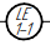
\includegraphics[width=0.08\textwidth]{imgs/PW2.1.png} \\ \hline

\textbf{Лампа розжарювання} – позначається у вигляді кола з хрестом. Може виступати ролі сигнальної. & 
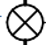
\includegraphics[width=0.08\textwidth]{imgs/PW2.2.png} \\ \hline

\textbf{Датчик витрат сировини} – позначається як \textbf{FE N-1}, що відображає потік матеріалу. & 
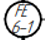
\includegraphics[width=0.08\textwidth]{imgs/PW2.3.png} \\ \hline

\textbf{Двигун конвеєра} – позначається символом \textbf{M N}, де N – порядковий номер двигуна. & 
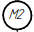
\includegraphics[width=0.1\textwidth]{imgs/PW2.4.png} \\ \hline

\textbf{Змішувач} – позначається числом \textbf{8} на технологічній схемі. & 
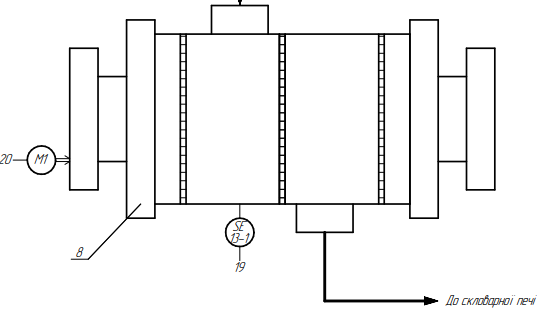
\includegraphics[width=0.3\textwidth]{imgs/PW2.5.png} \\ \hline

\textbf{Регулятор швидкості змішування} – позначений як \textbf{SE N-1}, що вказує на можливість зміни швидкості. & 
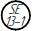
\includegraphics[width=0.1\textwidth]{imgs/PW2.6.png} \\ \hline

\textbf{Вимірювання показання реєстрації, регулювання подачі речовини в бункері} – позначений як \textbf{FIRS N-1}, що вказує на порядковий номер. & 
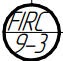
\includegraphics[width=0.1\textwidth]{imgs/PW2.7.png} \\ \hline

\textbf{Дистанційне ручне керування в бункері} – позначений як \textbf{HC N-1}, що вказує на порядковий номер. & 
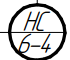
\includegraphics[width=0.1\textwidth]{imgs/PW2.8.png} \\ \hline

\textbf{Ручне вмикання/вимикання двигуна} – позначений як \textbf{HA}. & 
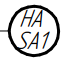
\includegraphics[width=0.1\textwidth]{imgs/PW2.9.png} \\ \hline
\end{tabular}
\end{table}

\newpage

\section*{Висновок}
Під час виконання роботи було детально проаналізовано функціональну схему автоматизації виробництва листового скла, вивчені стандарти позначень елементів та правила побудови схем автоматизації. Було ідентифіковано ключові елементи системи керування, контролю та регулювання процесів. Система автоматизації дозволяє забезпечити ефективне виробництво, контроль якості та безпеку виробничого процесу.


\section*{Відповіді на контрольні питання}

\begin{enumerate}
    \item \textbf{Для чого призначені ФСА?}\\
    Функціональні схеми автоматизації (ФСА) призначені для визначення функціональної структури окремих вузлів системи автоматичного контролю, керування або регулювання технологічним об'єктом, а також для оснащення його технічними засобами автоматизації.
    \item \textbf{Яким чином на ФСА зображують технологічне устаткування?}\\
    Технологічне устаткування на ФСА зображується у вигляді технологічної схеми, яка є графічним зображенням технологічного процесу або об'єкта в узагальнених рисах, з чітким уявленням про принцип роботи об'єкта та його взаємодію із технічними засобами автоматизації.
    \item \textbf{Які вимоги висуваються до графічних умовних позначень ТЗА?}\\
    Графічні умовні позначення технічних засобів автоматизації (ТЗА) на ФСА повинні відповідати вимогам ДСТУ Б А.2.4-3:2009 та інших відповідних стандартів, з дотриманням товщини ліній та розмірів позначень.
    \item \textbf{Які вимоги висуваються до умовних позначень трубопровідних комунікацій?}\\
    Умовні позначення трубопровідних комунікацій повинні відповідати стандартам, що регламентують їх зображення, включаючи лінії зв'язку, розділювальні риски та місця підключення.
    \item \textbf{Які вимоги до товщини ліній зв’язку на ФСА?}\\
    Товщина ліній зв'язку на ФСА повинна становити 0,2 – 0,3 мм.
    \item \textbf{Які вимоги до товщини ліній технологічного устаткування на ФСА?}\\
    Товщина ліній технологічного устаткування на ФСА має бути 0,5 – 0,6 мм.
    \item \textbf{Які вимоги до позиційних позначень ТЗА на ФСА?}\\
    Позиційні позначення ТЗА повинні відповідати вимогам стандартів і можуть бути цифровими або літерно-цифровими. Вони визначають номер функціональної групи та номер ТЗА у цій групі.
\end{enumerate}



\end{document}